\documentclass[12pt,a4paper]{article}
\usepackage{graphicx}
\usepackage[margin=2cm]{geometry} % Set the margins to 2cm on all sides
\usepackage{amsmath} % for advanced math typesetting
\usepackage{multicol}
\usepackage{enumitem}
\usepackage{url}
\usepackage{wrapfig}

\usepackage{tikz}
\usetikzlibrary{shapes, arrows.meta, positioning, fit, backgrounds}


\begin{document}

% Cover Page
\begin{titlepage}
    \begin{center}
        \vspace*{1cm}

        \includegraphics[width=0.75\textwidth]{UQLogo.jpg}
        
        \vspace{1.5cm}
        
        \textbf{\Large{School of Electrical Engineering and Computer Science}}
        
        \vspace{2.5cm}
        
        \textbf{\Large{PROJECT PROPOSAL}}
        
        \vspace{0.5cm}

        \textbf{\Large{Embedded Passive Radar Detection}}
        
        \vspace{2cm}
        
        \textbf{Flynn Kelly}\\
        47418589\\
        
        Commenced: 17/02/2024 - S1 2024\\
        Mode of study: Full-time - Internal\\
        Supervisor: Dr Konstanty Bialkowski
        
        \vfill
        
        \vspace{0.8cm}
        
        \Large{1}
        
    \end{center}
\end{titlepage}

% Table of Contents
\tableofcontents
\clearpage

% Beginning of Sections

\section{Introduction}
This proposal introduces the theory, motivations and planned process for the creation of an embedded passive radar detection system. 

\subsection{Topic and Relevance}
Passive radar detection technology is a class of radar detection whereby the radar system and by extension the radar receiver does not emit any radiation. Instead, it uses existing electromagnetic signals in the environment, such as television or radio broadcasts, to detect and track objects. Passive radar can be bistatic, whereby the transmitter and receiver are separate, or multistatic, where there are multiple receivers. The technology has been around since the early 20th century, but has only recently become feasible due to advances in digital signal processing and computing \cite{INTRO2017}.
\par
\vspace{0.5cm} 
\noindent The technology has a number of advantages over traditional radar systems. It is covert, as it does not emit any radiation, and is therefore difficult to detect and directly jam, leading to a concentrated interest from defence cirlces \cite{DTSO2009}. It is also relatively cheap, as it does not require a dedicated transmitter and hence has less energy consumption. Conversely, it has a number of disadvantages, such as a lower signal-to-noise ratio, and a requirement for a relatively large amount of computational power to process the received signals \cite{INTRO2017}.
\par
\vspace{0.5cm} 
\noindent Bistatic passive radar detection has a wide range of applications centered around situational awareness, including air traffic control, border security, and environmental monitoring. Embedding the passive radar technology is a relatively new field buoyed by recent and increasing developments in computational power on Internet of Things (IoT) devices \cite{IOTpassiveRadar}. This project aims to reinforce and build on existing technology by creating a low-cost, modular, small-scale embedded passive radar detection system. Moreover, this project will also explore the possibility of scaling up this bistatic setup to a multistatic system, and the potential advantages and disadvantages of such. 

\par
\vspace{0.5cm} 
\noindent More specifically, the project will focus on streamlining the signal processing and computational requirements of both the line of sight signal and the reflected target signal onto a singular embedded setup, without PC hardware. This will be achieved by using a combination of existing embedded IoT hardware, and through using existing DSP (digital signal processing) and radar filtering algorithms. Initially, the illuminator of opportunity selected is the DAB+ (digital audio broadcasting) signal, and the target signal will be aerial vehicles - most likely in the form of civillian passenger jets. Noting that a range of other terrestrial illuminator signals can be utilised, often tailored to specifically required use cases \cite{DABsignal}.

\subsection{Goals}
The primary goals of the project include the following, provided in order of logical progression;
\begin{itemize}
    \item Implement and investigate passive radar detection algorithms on high end computer architecture (PC) connected to SDR hardware and antenna for line of sight and target signal processing.
    \item Scaling down the passive radar detection system and associated algorithms to run on embedded IoT hardware, and investigate the computational and signal processing requirements, including the possible design of custom hardware such as peripheral functionality and printed circuit boards. A central feature of this specific goal is its ideally low cost nature.
    \item Verify functionality of low cost embedded passive radar detection system in a controlled environment against higher power computing results, and investigate the potential for scaling up to a multistatic system.
    \item Design and develop suitable housing for embdedded project implementation with ideal features such as modularity, portability and potential scaleability. 
\end{itemize}


\section{Background and Literature Review}

\subsection{Literature Review}
The below subsections reflect the neccessary research considerations for the project, and will be used to inform the project plan and optimize the implementation.

\subsubsection{Passive Radar Fundamentals}
The key and unique feature of passive radar is its utilisation of existing illuminators of opportunity, such as television or radio broadcasts, to detect and track objects. The technology has been around since the early 20th century, with modern interest accelerated due to the use passive radar systems on UHF TV signals and VHF FM radio tranmission systems in the 1980's \cite{FundamentalsPassiveRadar}. Equivalent terms used to describe passive radar include passive coherent location (PCL), and passive covert radar (PCR), parasitic radar, piggyback radar. Specifically, \textit{bistatic} radar refers to the distributed design of the transmitter and receiver, as opposed to classic \textit{monostatic} radar. As reflectd by Figure \ref{fig: topology} below, the turning parabolic of monostatic radar is able to receive both range and bearing of the signal echo, whereas passive bistatic radar measures time delay of the echos from the target, allowing doppler shift from the relative speed of the target to be measured.
\begin{figure}[htbp]
    \centering
    \includegraphics[width=0.8\textwidth]{monoBi.jpg}
    \caption{Monostatic (a) and bistatic (b) radar topologies \cite{IOTpassiveRadar}}
    \label{fig: topology}
\end{figure}
\par 
\vspace{0.5cm} 
\noindent The geometry of passive bistatic radar can be further explored and equations can be mapped accordingly, with the distance between the transmitter and receiver \textit{R} being determined by known quantities such as the baseline as reflected below in Figure \ref{fig:geometry}.

\begin{figure}[htbp]
    \centering
    \includegraphics[width=0.8\textwidth]{geomPR.jpg}
    \caption{Bistatic radar geometry \cite{FundamentalsPassiveRadar}}
    \label{fig:geometry}
\end{figure}

\par \vspace{0.5cm} 
\noindent The bistatic range \( R_R \) is given by:
\begin{equation}
R_R = \frac{(R_T + R_R)^2 - L^2}{2(R_T + R_R + L \sin \theta_R)}
\end{equation}

\noindent The Doppler shift \( f_D \) is given by the rate of change of the bistatic range sum:
\begin{equation}
f_D = \frac{1}{\lambda} \frac{d}{dt}(R_T + R_R) \xrightarrow{} f_D = \frac{2v}{\lambda} \cos \delta \cos(\frac{\beta}{2})
\end{equation}
In the case of this project, both the TX (illuminator of opportunity) and the RX (embedded passive detection system) will be static, and the target will be moving, simplifying the mathematical calculations as much as possible, resulting in the cos version of equation 2 above. The Doppler shift will be used to determine the speed of the target as well as its relative directional motion, and the range will be used to determine the distance of the target from the receiver.

\par \vspace{0.5cm} 
\noindent Another important feature of bistatic passive radar systems is its performance which can be equated through the bistatic radar equation, which is equivalently derived as the monostatic radar equation \cite{FundamentalsPassiveRadar}. 
\vspace{0.5cm} 
\begin{equation}
    \frac{P_r}{P_n} = \frac{P_t G_t}{4\pi R_T^2} \cdot \sigma_B \cdot \frac{1}{4\pi R_R^2} \cdot \frac{G_r \lambda^2}{4\pi} \cdot \frac{1}{k T_0 B F}
\end{equation}
Where:
\begin{multicols}{2}
    \begin{itemize}
    \item \( P_r \) is the received target echo power.
    \item \( P_n \) is the receiver noise power.
    \item \( P_t \) is the transmit power.
    \item \( G_t \) is the transmit antenna gain.
    \item \( R_T \) is the transmitter-to-target range.
    \item \( \sigma_B \) is the target bistatic radar cross section.
    \item \( R_R \) is the target-to-receiver range.
    \item \( G_r \) is the receive antenna gain.
    \item \( \lambda \) is the signal wavelength.
    \item \( k \) is Boltzmann’s constant (\( 1.38 \times 10^{-23} \) JK\(^{-1}\)).
    \item \( T_0 \) is the noise reference temperature.
    \item \( B \) is the receiver effective bandwidth.
    \item \( F \) is the receiver effective noise figure.
    \end{itemize}
\end{multicols}
\noindent The denominator of the bistatic radar equation includes the term \( \frac{1}{R_T^2 R_R^2} \).This term implies that with omnidirectional antenna patterns, the contours of constant signal-to-noise ratio (SNR) are described by the equation \( R_T R_R = \text{constant} \), which represents Ovals of Cassini. In the case of directional antennas, these contours are altered. Moreover, the signal-to-noise ratio is minimized when the target is equidistant from the transmitter and receiver (\( R_T = R_R \)), and maximized when the target is closer to either the transmitter or receiver \cite{FundamentalsPassiveRadar}.

\par \vspace{0.5cm} 
\noindent Ideally this project would process just the target signal, however, that is an unrealistic expectation due to the presence of clutter. Clutter refers to unwanted signal that eminates from objects in the natural environemnt such as buildings, trees and ground \cite{zhang2023intelligent}. This process of target signal clutter suppression and its impact on range doppler mapping will be discussed later in the literature review.  

\subsubsection{Illuminators of Opportunity}
The illuminator of opportunity is the signal that is used to illuminate the target, and is the primary source of the signal that is received by the passive radar system. The illuminator of opportunity can be any signal that is transmitted through the air, such as television or radio broadcasts, and can be tailored to the specific requirements of the passive radar system. Griffiths and Baker outline the three key paramaters when selecting an illuminator \cite{INTRO2017}:
\begin{enumerate}[label=\arabic*.]
    \item The \textbf{Power Density} at the target: It refers to the strength of the signal (in Watts per square meter) that reaches the target area from the illuminator. Higher power density can improve detection performance due to a stronger return signal.
    \item The \textbf{Nature of the Waveform}: This includes the waveform's properties, such as bandwidth and modulation, which can affect the radar's resolution and ability to distinguish between targets and clutter.
    \item The \textbf{Coverage}: The spatial area over which the illuminator's signal is spread. Adequate coverage is essential to ensure the target is within the illuminator's effective range.
\end{enumerate}
Illuminator signals are not limited to terrestrial signals, and can also include signals from satellites, and can be tailored to the specific requirements of the passive radar system. The illuminator of opportunity selected for this project is the DAB+  signal, and the target signal will be aerial vehicles - most likely in the form of civillian passenger jets. The DAB+ signal was selected due to its high power density, and its relatively high bandwidth, which can be used to improve the radar's resolution and ability to distinguish between targets and clutter. Moreover, the geographical proximity of a DAB+ transmitter at Mt Cootha to the University of Queensland, St Lucia campus, makes it an ideal choice for the project.
\par \vspace{0.5cm} 
\noindent ****** DIRECT SIGNAL INTERFERENCE??? *******

\par \vspace{0.5cm} 
\noindent Typical characteristics of Australian DAB+ signals include frequency of just over 200MHz, bandwidth of approximately 1.5MHz, and a minimal output power of 10kW effective radiated power (ERP), consequently covering a large area \cite{DABfeatures}. These digital signals employ a modulation scheme called COFDM (coded orthogonal frequency division multiplexing), which is a form of multi-carrier modulation that is robust against multipath interference \cite{INTRO2017}. COFDM works by dividing the signal into multiple, simultaneous streams which are orthogonal to each other, modulated at a different frequency, maximising robust signal propogation. This is particularly useful in the context of passive radar, as it allows for the target and reference signal to be received by the passive radar system even if it has been reflected off multiple surfaces, such as buildings or trees.

\par \vspace{0.5cm} 
\noindent All of the above features result in DAB signals being condusive for ambiguity function performance (analyzed in further detail below). This can mainly be attributed to the relatively wide bandwidth of DAB enabling good resolution, constant DAB envelope stemming from COFDM protocol, and the multipath resistance \cite{DABambiguity}.
\subsubsection{Range Doppler Mapping}
Range doppler mapping is a technique used to determine the distance and relative velocity of targets by analyzing the frequency shift (Doppler shift) and time delay of the received signals after they bounce off the targets. The signal response of a target at a particular range and velocity can be predicted by the ambiguity function seen in equation 4 \cite{INTRO2017}. 
\begin{equation}
    \chi(\tau, f) = \int s_1(t) s_2^*(t - \tau) e^{j2\pi f t} \, dt
\end{equation}
Where:
\begin{multicols}{2}
\begin{itemize}
\item \( \chi(\tau, f) \) is the ambiguity function.
\item \( \tau \) is the time delay.
\item \( f \) is the Doppler frequency.
\item \( s_1(t) \) is the transmitted signal.
\item \( s_2(t) \) is the received signal.
\item \( s_2^*(t - \tau) \) is the complex conjugate of the received signal, time-shifted by \( \tau \).
\item \( e^{j2\pi f t} \) is the complex exponential representing the Doppler shift.
\item The integral is taken over all time \( t \).
\end{itemize}
\end{multicols}
\noindent The ambiguity function can be plotted, thereby visualising resolution, sidelobe patterns and any discrepancies in range and doppler. This is especially important for passive bistatic radar, whereby waveforms are not explicitly designed for radar and the geometry also has an impact \cite{FundamentalsPassiveRadar}. Hughes visualises the geometry considerations and potential flaws of passive bistatic below in Figure \ref{fig:ambiguity}.
\begin{figure}[htbp]
    \centering
    \includegraphics[width=0.35\textwidth]{ambiguity.jpg}
    \caption{Geometry and ambiguity function \cite{FundamentalsPassiveRadar}}
    \label{fig:ambiguity}
\end{figure}
\par \vspace{0.5cm} 
\noindent Understanding the link between geometric configuration and theoretical signal properties, the practical manifestation of the ambiguity function is range doppler mapping. As shown in Figure \ref{fig:rangeDoppler}, the map is a heat map and is derived with filters for noise minimsation, allowing for the visualisation of the target signal with minimal clutter. 
\begin{figure}[htbp]
    \centering
    \includegraphics[width=0.5\textwidth]{rangeDoppler.jpg}
    \caption{Example of range doppler map for WiFi PBR \cite{FundamentalsPassiveRadar}}
    \label{fig:rangeDoppler}
\end{figure}
\par  
\noindent In the case of this project, the time delay will be utilised to calculate the bistatic range (x axis) and the Doppler shift will be used to calculate the relative velocity of the target (y axis). In summary, ambiguity function and subequent range doppler mapping will be vital for mapping the DAB+ signal characteristics for given geometry and motion of the surveilled target.
\subsubsection{Radio Hardware}
Given the low cost aims of this project, hardware cost will majorly impact the overall cost. Luckily, the proliferation of Software Defined Radio (SDR) has enabled low cost hardware modules enabling easy access to radio frequency (RF) signals \cite{SDRtheory}. The most popular SDR module is the RTL-SDR, which is a USB dongle that can be used to receive and decode a wide range of RF signals. The RTL-SDR is based on the Realtek RTL2832U chipset, and has a frequency range of 24MHz to 1.7GHz, and a bandwidth of 3.2MHz. The RTL-SDR is also relatively cheap, with a price of around \$40 AUD. The RTL-SDR is also compatible with a wide range of software, including MATLAB, and GNU radio \cite{SDRdongle}. Given the digital nature of the DAB+ signal, the direct reference signal and the target surveillance signal can in theory be sampled by a singular RTL2832U module as shown by Barrot et.al \cite{DABsingleRadar}.
\par  
\noindent ****** NEED TO EXPLORE REONSTRUCTION OPTIONS / CONFIG \(\rightarrow\)reference signal from surveillance signal *****
\par  
\noindent Regardless of sampling hardware architecture, based on previous studies and the nature of the DAB+ signal and modulation framework, a sampling rate of 2.048\,MS/s is prudent \cite{IOTpassiveRadar}.

\subsubsection{IoT Architecture}
The IoT architecture in the scope of this project refers to the computational platforms utilised to undertake the digital signal processing which then maps to tracking and detection of the target. Existing studies have demonstrated the ability of off the shelf laptops \cite{FMlowCost}, and there is a few studies that use IoT platforms for FM signal processing \cite{IOTpassiveRadar}. The vital consideration when exploring hardware is the DSP requirements of the bistatic passive detection process (explored further in the next section).
\par \vspace{0.5cm} 
\noindent The broad scope capability requirements of the computational platform is identified below in Figure \ref{fig:block_diagram}, which also highlights the division of responsibility between system hardware (IoT computer and SDR hardware).

\begin{figure}[htbp]
    \centering
    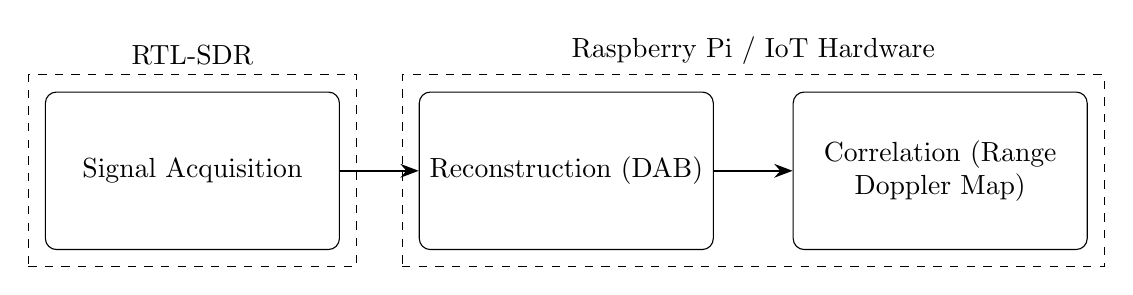
\begin{tikzpicture}[
        block/.style={
          rectangle,
          draw,
          text width=3.5cm,
          align=center,
          rounded corners,
          minimum height=2cm
        },
        line/.style={-Stealth, thick},
        dottedBox/.style={
          rectangle,
          draw,
          dashed,
          inner sep=6pt,
          label=above:#1
        }
    ]
    
    % Define the nodes
    \node[block] (signalAcq) {Signal Acquisition};
    \node[block, right=of signalAcq] (reconstruct) {Reconstruction (DAB)};
    \node[block, right=of reconstruct] (correlate) {Correlation (Range Doppler Map)};
    
    % Connect the nodes
    \draw[line] (signalAcq) -- (reconstruct);
    \draw[line] (reconstruct) -- (correlate);
    
    % Dotted boxes
    \node[dottedBox=RTL-SDR, fit=(signalAcq)] {};
    \node[dottedBox=Raspberry Pi / IoT Hardware, fit=(reconstruct) (correlate)] {};
    
    \end{tikzpicture}
    \caption{Block diagram showing the high level hardware process}
    \label{fig:signal_processing_flow}
    \end{figure}
    
\noindent A possible IoT device that could be used, and has evidence of previous use as demonstrated by Moser et. al \cite{IOTpassiveRadar} is the Raspberry Pi platform, which despite having increased processing times demonstrated its functionality. An alternate, higher powered choice in which Sednall demonstrated is the higher powered Nvidia Jetson, which includes faster processing times due to its quad core architecture \cite{FMlowCost}. The price for these options is \$60 compared to \$250 respectively. Ultimately, the choice of embedded IoT hardware for the project can be reduced to the trade off between low cost and processing power, and will be a key consideration in the project plan. Furthermore, there is possibility to design custom hardware to optimise for processing speeds and project cost, for example, a PCB extension utilising a Raspberry Pi with DSP IC chips and/or custom user buttons.



\subsubsection{Signal Processing and Algorithms} 

\begin{wrapfigure}{r}{0.6\textwidth} % This places the figure on the right and occupies 60% of the text width
    \centering
    \includegraphics[width=0.43\textwidth]{DSPprocess.png}
    \caption{Main steps of signal processing \cite{detectionDABmodulation}}
    \label{fig:DSP}
\end{wrapfigure}

Broadly, the goal of the signal processing for this project is to extract a range doppler map from the received reference and surveillance signals. In order to achieve this, a range of steps are required to be undertaken. A range of literature exists for the signal processing of FM illuminator of opportunity signals, including Batches algorithm \cite{DSPfm}. However, given the nature of DAB and its COFDM modulation (explored above), filtering and synchronisation can be replaced with reconstruction of the surveillance signal \cite{DSPdab}. The use of a singular antenna is affirmed by Schupbach et. al \cite{UAVdab} who utilised DAB passive radar to track micro-UAVs.

\par \vspace{0.5cm} 
\noindent Figure \ref{fig:DSP} from Poullin \cite{detectionDABmodulation} shows the main steps of the required signal processing, which includes signal acquisition, reconstruction, and correlation. 

\par \vspace{3.5cm} 
\noindent The scope of this project involves branches 1 through 3, with target analysis representing a logical extension for a more complicated version of the project. 
\par \vspace{0.5cm} 
\noindent ****** NEED MORE RESEARCH AND UNDERSTANDING OF DECODING AND DEMODULATION OF DAB \(\rightarrow\) CORRELATE / INTEGRATE FOR RDM ?*****
\par \vspace{0.5cm} 
\noindent Once signal has been demodulated, according to Moser et. al, FFT the size of 2048 for the range domain and 512 for the doppler domain can be computed \cite{IOTpassiveRadar}, see Figure \ref{fig:FFT}. NEED MORE UNDERSTANDING HERE!!!
\begin{figure}[htbp]
    \centering
    \includegraphics[width=0.8\textwidth]{FFT.png}
    \caption{Correlation and FFT for Range Doppler Mapping \cite{IOTpassiveRadar}}
    \label{fig:FFT}
\end{figure}
\par \vspace{0.5cm} 
\noindent Logically, the step above relfects the most computationally intensive process of the project .... EXPLAIN hardware considerations!!!

\subsection{Pilot Studies \& Existing PBR Technology}
Discuss silentium defence Maverick-M silent radar, IoT example, drone embedded example. SILENT SENTRY, DTSO



\section{Project Plan}
\subsection{Aim of Project}
\subsection{Milestones}
\subsection{Timeline}


% References (You will need to use BibTeX to manage your references)
% The bibliography style can be changed to suit your needs
\newpage
\bibliographystyle{plain}
\bibliography{references}

\end{document}
